\documentclass{article}
\usepackage{tikz}
\usetikzlibrary{arrows.meta, decorations.pathmorphing}

\begin{document}

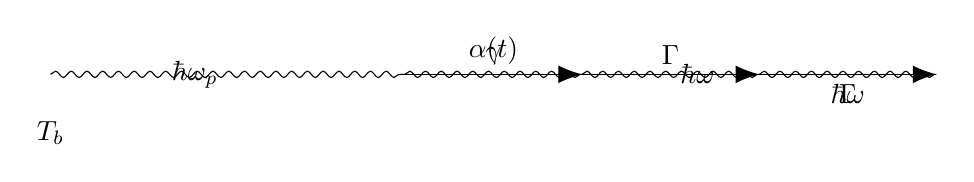
\begin{tikzpicture}[scale=1.5]
    % Draw the wavy lines
    \draw[decorate, decoration={snake, amplitude=.4mm, segment length=2mm}] (-3,0) -- node[left] {$\hbar\omega_p$} (0,0);
    \draw[decorate, decoration={snake, amplitude=.4mm, segment length=2mm}] (0,0) -- node[above] {$\alpha(t)$} (1.5,0);
    \draw[decorate, decoration={snake, amplitude=.4mm, segment length=2mm}] (1.5,0) -- node[right] {$\hbar\omega$} (3,0);
    \draw[decorate, decoration={snake, amplitude=.4mm, segment length=2mm}] (3,0) -- node[below] {$\hbar\omega$} (4.5,0);

    % Draw the arrows
    \draw[-{Latex[length=3mm]}] (0,0) -- node[above] {$\gamma$} (1.5,0);
    \draw[-{Latex[length=3mm]}] (1.5,0) -- node[above] {$\Gamma$} (3,0);
    \draw[-{Latex[length=3mm]}] (3,0) -- node[below] {$\Gamma$} (4.5,0);

    % Draw the labels
    \node at (-3,-0.5) {$T_b$};
    \node at (4.5,-0.5) {};
\end{tikzpicture}

\end{document}